%%%%%%%%%%%%%%%%%%%%%%%%%%%%%%%%%%%%%%%%%
% fphw Assignment
% LaTeX Template
% Version 1.0 (27/04/2019)
%
% This template originates from:
% https://www.LaTeXTemplates.com
%
% Authors:
% Class by Felipe Portales-Oliva (f.portales.oliva@gmail.com) with template 
% content and modifications by Vel (vel@LaTeXTemplates.com)
%
% Template (this file) License:
% CC BY-NC-SA 3.0 (http://creativecommons.org/licenses/by-nc-sa/3.0/)
%
%%%%%%%%%%%%%%%%%%%%%%%%%%%%%%%%%%%%%%%%%

%----------------------------------------------------------------------------------------
%	PACKAGES AND OTHER DOCUMENT CONFIGURATIONS
%----------------------------------------------------------------------------------------

\documentclass[
	12pt, % Default font size, values between 10pt-12pt are allowed
	%letterpaper, % Uncomment for US letter paper size
	spanish, % Uncomment for Spanish
]{fphw}

% Template-specific packages
\usepackage[utf8]{inputenc} % Required for inputting international characters
\usepackage[T1]{fontenc} % Output font encoding for international characters
\usepackage{mathpazo} % Use the Palatino font
\usepackage{amsmath, amssymb}
\usepackage{graphicx} % Required for including images
\usepackage{booktabs} % Required for better horizontal rules in tables
\usepackage{cancel}
\usepackage{listings} % Required for insertion of code

\usepackage{enumerate} % To modify the enumerate environment

\newcommand{\vu}{\vec{u}}
\newcommand{\vv}{\vec{v}}
\newcommand{\vw}{\vec{w}}



%----------------------------------------------------------------------------------------
%	ASSIGNMENT INFORMATION
%----------------------------------------------------------------------------------------

\title{UNIDAD 4: Cuestiones de teoría a desarrollar y saber} % Assignment title

\author{Javier Ribal del Río} % Student name

\date{Curso 2023-24}
\institute{Colegio Salesianos San Juan Bosco} % Institute or school name

\class{Matemáticas II} % Course or class name

\professor{José Antonio Chaveli} % Professor or teacher in charge of the assignment

%----------------------------------------------------------------------------------------

\begin{document}

\maketitle % Output the assignment title, created automatically using the information in the custom commands above

%----------------------------------------------------------------------------------------
%	ASSIGNMENT CONTENT
%----------------------------------------------------------------------------------------

\section*{1}

\begin{problem}
	Relación entre rango de un conjunto de vectores y su posición geométrica
	(Característica geométrica)\end{problem}


%------------------------------------------------

\subsection*{Respuesta} El rango de un grupo de vectores es la cantidad de ellos que son linealmente independientes mientras que la posición geometrica es la cantidad del espacio que podemos alcanzar realizando combinaciones lineales entre estos vectores. Cuanto mayor sea el rango de el conjunto de vectores (base) a más posición geométricas podremos acceder.

%----------------------------------------------------------------------------------------

\section*{2}

\begin{problem}
	Producto escalar: Definición, consecuencias, propiedades, expresión analítica
	en una base ortonormal y aplicaciones geométricas.	
	
\end{problem}

%------------------------------------------------

\subsection*{Respuesta}

\begin{gather*}
	V_3 \times V_3 \rightarrow \mathbb{R}\\
	\vec{u}, \vec{v} \rightsquigarrow \vec{u} \bullet \vec{v} = |\vec{u}|\cdot |\vec{v}| \cdot \cos(\alpha)
\end{gather*}

Consecuencias:

\begin{flalign*}
	& 1) \alpha \in [0,90 ) \leftrightarrow \vec{u} \bullet \vec{v} > 0\\
	& 2) \alpha = 90 \leftrightarrow \vec{u} \bullet \vec{v} = 0 \leftrightarrow \vec{u} \perp \vec{v} \\
	& 3) \alpha \in  (90, 180] \leftrightarrow \vec{u} \bullet \vec{v} < 0 \\
	& 4) - |\vec{u}| \cdot |\vec{v}| \leq \vec{u} \bullet  \vec{v} \leq | \vec{u} | \cdot | \vec{v}| \\
	& 5) \vec{u} \bullet \vec{u} = |\vec{u}| \cdot |\vec{u}| \cdot \cancel{\cos(\alpha)}^1 \rightarrow |\vec{u}|^2 = \vec{u} \bullet \vec{u} \rightarrow |\vec{u}|= \sqrt{\vec{u} \bullet \vec{u}}
\end{flalign*}


 Propiedades operativas: 

\begin{flalign*}
	& 1) \vec{u} \bullet \vec{v} = \vec{v} \bullet \vec{u} \\
	& 2) \vec{u} \bullet \vec{u} \geq 0 \\
	& 3) \vec{u} \bullet (\vec{v} +\vec{w}) = \vec{u} \bullet \vec{v} + \vec{u} \bullet \vec{w}\\
	& 4) k \cdot (\vec{u} \bullet \vec{w}) = (k \cdot \vec{u}) \bullet \vec{v} = \vec{u} \bullet (k \cdot \vec{v})
\end{flalign*}
%----------------------------------------------------------------------------------------

Expresión analítica en base canónica:

\begin{gather*}
	\vec{u}=(u_1,u_2,u_3);\vec{v} =(v_1,v_2,v_3)\\
	\vec{u} \bullet \vec{v} = u_1 \cdot v_1 + u_2 \cdot v_2 + u_3  \cdot v_3
\end{gather*}
Ejemplo $\vec{u} = (2,-3,1); \vec{v} = (1,3,2); \vec{u} \bullet \vec{v} = 9$.\\

El producto escalar tiene varias aplicaciones geométricas, en primer lugar lo podemos utilizar para comprobar la perpendicularidad de dos vectores ya que su porducto escalar será 0. En segundo lugar, lo podemos utilizar para calcular el módulo de un vector. Por último, también se puede utilizar para calcular el ángulo de dos vectores.


\section*{3}

\begin{problem}
	Producto vectorial: Definición, consecuencias, propiedades, expresión analítica
	en una base ortonormal y aplicaciones geométricas.	
	
\end{problem}

%------------------------------------------------

\subsection*{Respuesta}

\begin{gather*}
	V_3 \times V_3 \rightarrow V_3\\
	\vec{u}, \vec{v} \rightsquigarrow \vec{u} \times \vec{v}\\
\end{gather*}
\begin{itemize}
	\item Dirección: $(\vec{u} \times \vec{v}) \perp \vec{u}, (\vec{u} \times \vec{v}) \perp \vec{v}$\\
	\item Sentido: $\vec{u} \times \vec{v}, \vec{v} \times \vec{u}$ tendrán sentidos opuestos\\
	\item Módulo: $|\vec{u} \times \vec{u} | = |\vec{u}| \cdot |\vec{v}| \cdot \sin(\alpha)$\\
\end{itemize}

Consecuencias:

\begin{enumerate}
	\item $\alpha \in \{0,180\} \rightarrow \vec{u} \times \vec{w} = \vec{o}$ ($\vec{u}$ y $\vec{v}$ no son linealmente independientes)
	\item $\vec{u} = \vec{o} \rightarrow \vec{u} \times \vec{v} = \vec{o}$
\end{enumerate}


Propiedades operativas:

\begin{enumerate}
	\item Si $\vec{u}$ y $\vec{v}$ tienen la misma dirección, $\vec{u} \times \vec{v} = \vec{o}$
	\item $\vec{u} \times \vec{v} = -(\vec{v} \times\vec{u})$
	\item $(\vec{u} \times \vec{v}) \cdot \vec{u} = 0; (\vec{v} \times \vec{u}) \cdot \vec{u} = 0$
	\item $\vec{u} \times (\vec{v} + \vec{w}) = \vec{u} \times \vec{v} + \vec{u} \times \vec{w}$
	\item $k\cdot(\vec{u} \times \vec{v}) =( k \cdot \vec{u}) \times \vec{v}= \vec{u} \times (k \cdot\vec{v})$\\
\end{enumerate}

Expresión analítica en base canónica:

\begin{gather*}
	\vec{u}=(u_1,u_2,u_3);\vec{v} =(v_1,v_2,v_3)\\
	\vec{u} \times \vec{v} = 
	\begin{vmatrix}
		\vec{i} & \vec{j} & \vec{k} \\
		u_1 & u_2 & u_3\\
		v_1 & v_2 & v_3 \\
	\end{vmatrix} = ( , , ,)
\end{gather*}

El producto vectorial tiene varias aplicaciones geométricas, en primer lugar lo podemos utilizar para encontrar vectores perpendicualres a otros dos, en segundo lugar para calcular el vector normal ($\vec{n}$) de un plano y por último para encontrar el arear del paralelogramo que forman los vectores $\vec{u}$ y $\vec{v}$.



\section*{4}

\begin{problem}
	
Producto mixto: Definición, consecuencias, propiedades, expresión analítica en
una base ortonormal y aplicaciones geométricas.
\end{problem}

\subsection*{Respuesta}

\begin{gather*}
	V_3 \times V_3 \times V_3 \rightarrow \mathbb{R}\\
	\vec{u},\vec{v},\vec{w} \rightsquigarrow [\vec{u},\vec{v},\vec{w}] =  \vec{u} \cdot (\vec{v} \times \vec{w})
\end{gather*}


Consecuencias:

$[\vu,\vv,\vw] = 0$

\begin{enumerate}
	\item Si $\vu, \vv$ o $\vw$ son el vector nulo $\vec{o}$
	\item Si $\vv$ y $\vw$ tienen la misma dirección
	\item Si $\vu \perp (\vv \times \vw)$
	\item Si $\vu, \vv$ y $\vw$ con coplanarios
\end{enumerate}

Propiedades:

\begin{enumerate}
	\item $[\vu,\vv,\vw] = [\vv,\vw,\vu] = [\vw,\vu,\vv]$
	\item $[\vu,\vv,\vw] = - [\vv,\vu,\vw] = - [\vu,\vw,\vv] = - [\vw,\vv,\vu]$
	\item $[\vec{u_1} + \vec{u_2}, \vv,\vw] = [\vec{u_1},\vv,\vw] + [\vec{u_2},\vv,\vw]$
	\item $k[\vu,\vv,\vw] = [k\vu,\vv,\vw] = [\vu,k\vv,\vw] = [\vu,\vv,k\vw], \forall k \in \mathbb{R}$
\end{enumerate}

Expresión analítica en base canónica:

\begin{gather*}
	[\vu,\vv,\vw] = 
	\begin{vmatrix}
		u_1 & u_2 & u_3\\
		v_1 & v_2 & v_3\\
		w_1 & w_2 & w_3 \\
	\end{vmatrix}
\end{gather*}

A través del producto mixto podemos calcular directamente el area del paralelepipedo que forman los tres vectores. También lo podemos utilizar para sever si los tres vectores son coplanarios

\section*{5}

\begin{problem}
	Relación entre las propiedades de los determinantes y la del producto vectorial
\end{problem}
\subsection*{Respuesta}
\begin{itemize}
	\item  $\vec{u} \times \vec{v} = \vec{o} \leftrightarrow \alpha = 180º \cdot k, k \forall \in \mathbb{R}\leftrightarrow \vv$ es una combinación lineal\\
	\item $\vec{u} \times \vec{v} = -(\vec{v} \times\vec{u}) \leftrightarrow
	 \begin{vmatrix}
		\vec{i} & \vec{j} & \vec{k} \\
		u_1 & u_2 & u_3\\
		v_1 & v_2 & v_3 \\
	\end{vmatrix} = - 
	\begin{vmatrix}
		\vec{i} & \vec{j} & \vec{k} \\
		u_1 & u_2 & u_3\\
		v_1 & v_2 & v_3 \\
	\end{vmatrix} $
	\item $\vec{u} \times (\vec{v} + \vec{w}) = \vec{u} \times \vec{v} + \vec{u} \times \vec{w} \leftrightarrow 
	 \begin{vmatrix}
		\vec{i} & \vec{j} & \vec{k} \\
		u_1 & u_2 & u_3\\
		v_1 + w_1 & v_2 + w_2 & v_3 +w_3 \\	\end{vmatrix} = 
	\begin{vmatrix}
		\vec{i} & \vec{j} & \vec{k} \\
		u_1 & u_2 & u_3\\
		v_1 & v_2 & v_3 \\
	\end{vmatrix} +
	\begin{vmatrix}
		\vec{i} & \vec{j} & \vec{k} \\
		u_1 & u_2 & u_3\\
		w_1 & w_2 & w_3 \\
	\end{vmatrix}$

	\item $k\cdot(\vec{u} \times \vec{v}) =( k \cdot \vec{u}) \times \vec{v}= \vec{u} \times (k \cdot\vec{v}) \leftrightarrow 
	k \begin{vmatrix}
		\vec{i} & \vec{j} & \vec{k} \\
		u_1 & u_2 & u_3\\
		v_1 & v_2 & v_3 \\
	\end{vmatrix} =  
	\begin{vmatrix}
		\vec{i} & \vec{j} & \vec{k} \\
		ku_1 & ku_2 & ku_3\\
		v_1 & v_2 & v_3 \\
	\end{vmatrix}=
	\begin{vmatrix}
		\vec{i} & \vec{j} & \vec{k} \\
		u_1 & u_2 & u_3\\
		kv_1 & kv_2 & kv_3 \\
	\end{vmatrix} $
	\\


\end{itemize}

\section*{6}
\begin{problem}
	Relación entre las propiedades de los determinantes y la del producto mixto
\end{problem}
\subsection*{Respuesta}
\begin{enumerate}
	\item $[\vu,\vv,\vw] = [\vv,\vw,\vu] = [\vw,\vu,\vv] \rightarrow$ Podemos cambiar el orden de las lineas de los determinantes cambiando el signo, en este caso se hacen dos cambios por lo que el signo se cambia a negativo, y luego otra vez a positivo
	\item $[\vu,\vv,\vw] = - [\vv,\vu,\vw] = - [\vu,\vw,\vv] = - [\vw,\vv,\vu] \rightarrow$ Al igual que en la anterior, cambiar el orden de los vectores cambia el orden de las lineas que cambia el signo, en este caso se realiza uno o tres cambios
	\item $[\vec{u_1} + \vec{u_2}, \vv,\vw] = [\vec{u_1},\vv,\vw] + [\vec{u_2},\vv,\vw] \leftrightarrow =
	\begin{vmatrix}
			u_{1x} + u_{2x} & u_{1y} + u_{2y} & u_{1z}+ u_{2z}\\
			v_x & v_y & v_z\\
			w_x & w_y & w_z\\	
	\end{vmatrix}
	=
	\begin{vmatrix}
			u_{1x} & u_{1y} & u_{1z}\\
			v_x & v_y & v_z\\
			w_x & w_y & w_z\\	
	\end{vmatrix}
	+
	\begin{vmatrix}
			u_{2x} & u_{2y} & u_{2z}\\
			v_x & v_y & v_z\\
			w_x & w_y & w_z\\	
	\end{vmatrix}$
	\item $k[\vu,\vv,\vw] = [k\vu,\vv,\vw] = [\vu,k\vv,\vw] = [\vu,\vv,k\vw], \forall k \in \mathbb{R} \leftrightarrow k 
	\begin{vmatrix}
	u_1 & u_2 & u_3\\
	v_1 & v_2 & v_3\\
	w_1 & w_2 & w_3\\	
	\end{vmatrix}
	= 
	\begin{vmatrix}
		ku_1 & ku_2 & ku_3\\
		v_1 & v_2 & v_3\\
		w_1 & w_2 & w_3\\	
	\end{vmatrix}
	=
	\begin{vmatrix}
			u_1 & u_2 & u_3\\
			kv_1 & kv_2 & kv_3\\
			w_1 & w_2 & w_3\\	
	\end{vmatrix}
	=
	\begin{vmatrix}
			u_1 & u_2 & u_3\\
			v_1 & v_2 & v_3\\
			kw_1 & kw_2 & kw_3\\	
	\end{vmatrix}$

\end{enumerate}

\section*{7}
\begin{problem}
	Dados dos vectores, relación entre el módulo del producto vectorial, área del
paralelogramo definido, área del triangulo definido y sus correspondientes
alturas respecto un lado determinado.
\end{problem}

\subsection*{Respuesta}

El area del paralelogramo (ABCD) que forman dos vectores corresponde con el módulo del producto vectorial de estos por lo que:

\begin{gather*}
	A_{Paralelogramo} = b \cdot h = |\vu \times \vv| = |\vu| \cdot |\vv| \cdot \sin(\alpha) \\
	h = AD \cdot \sin(\alpha) = |\vv| \cdot \sin(\alpha)\\
\end{gather*}

Además el area del triángulo es la mitad del paralelogramo que forman los dos vectores:

\begin{gather*}
A_{Tri\acute{a}ngulo} = \frac {1} {2} \cdot b \cdot h = \frac{1}{2} \cdot |\vu \times \vv| = \frac{1}{2} \cdot |\vu| \cdot |\vv| \cdot \sin(\alpha)\\
\end{gather*}

Al igual que en el ejemplo anterior, el módulo del vector $\vu$ corresponde a la base y $|\vv|\sin(\alpha)$ corresponde a la altura de dicho lado, aun así esto no es importante porque por la propiedad conmutativa de la multiplicación $|\vv|$ podría ser la base y $|\vu|\sin(\alpha)$ la altura.\\

Poniendo un triángulo ABC, siendo $\vu$ el vector que corresponde con el lado $c$ y $\vv$ el que corresponde con el lado $b$:

\begin{itemize}
	\item Altura del lado $a$: $h_a= |\vu|\cdot\sin(\hat{B})$
	\item Altura del lado $b$: $h_b= |\vu|\cdot\sin(\hat{A})$
	\item Altura del lado $c$: $h_c= |\vv|\cdot\sin(\hat{A})$
\end{itemize}


\section*{8}
\begin{problem}
	Dado tres vectores: relación entre el producto \textbf{mixto}, volumen del
tetraedro y paralelepípedo definidos, la altura dada una cara.
\end{problem}

\begin{center}
	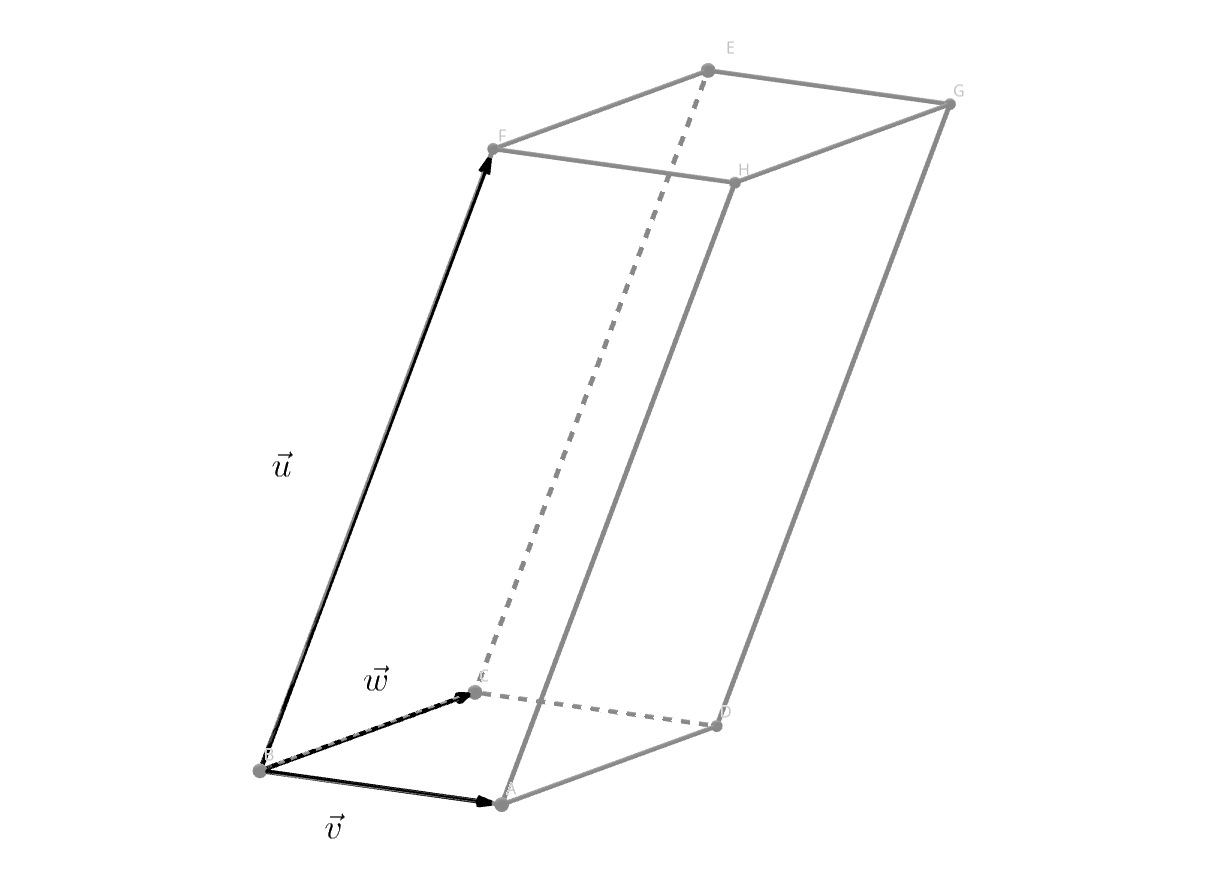
\includegraphics[width=0.5\columnwidth]{Paralelepipedo.png} % Example image
\end{center}

Un paralelepipedo es un poliedro compuesto por seis caras, la formula de su volumen es la siguiente:

\begin{gather*}
	V_{paralelep\acute{i}pedo} = S_{base} \cdot h
\end{gather*}

Podemos observar que los vectores $\vv$ y $\vw$ corresponden con dos de las aristas de la base, por lo que para calcular la superficie de la base podemos recuerir al producto vectorial. Además, el vector resultante del producto vectorial de $\vv$ y $\vw$ es perpendicular a la base y  coincidente con la altura  ya  como disponemos del vector $\vu$ podemos, a través de las funciones trigonometricas, determinar la altura del paralelepipedo. Siendo $\alpha$ el ángulo formado entre $\vv \times \vw$ y $\vu$.

\begin{gather*}
	S_{base} = |\vv \times \vw|\\
	\cos(\alpha) = \frac{h}{|\vu|} \leftrightarrow h=|\vu| \cdot \cos(\alpha) 
\end{gather*}
 

\begin{center}
	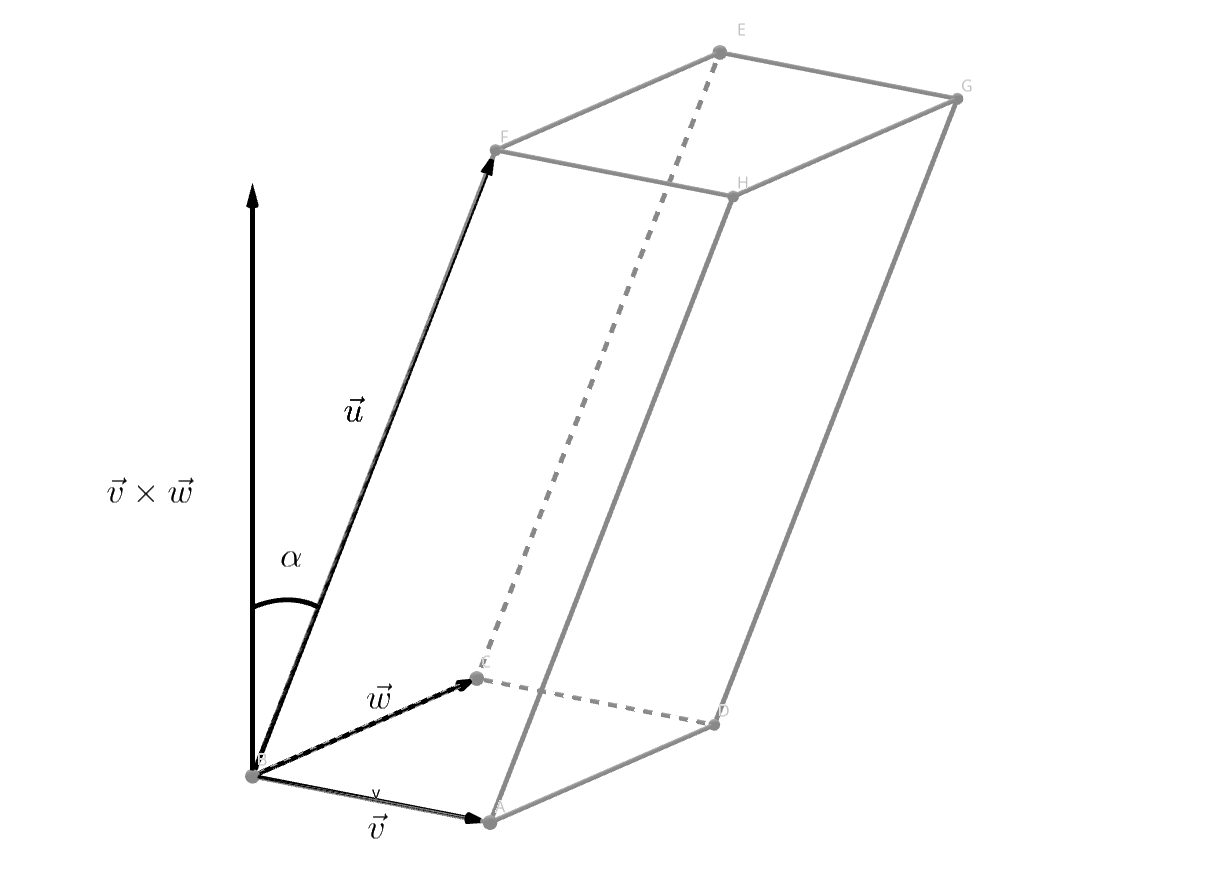
\includegraphics[width=0.6\columnwidth]{geogebra-export.png} % Example image
\end{center}

Si juntamos todo lo anterior descubrimos que el area del paralelepipedo coincide con el producto mixto de los tres vectores, ya que, sintéticamnete, el producto mixto es el producto escalar de un vector con el resultado de un producto vectorial.

\begin{gather*}
	V_{paralelep\acute{i}pedo} = S_{base} \cdot h = |\vv \times \vw| \cdot |\vu| \cdot \cos(\alpha) = |\vu| \cdot|\vv \times \vw| \cdot \cos(\alpha)=[\vu,\vv,\vw]\\
	V_{paralelep\acute{i}pedo} = [\vu,\vv,\vw]
\end{gather*}


Respecto al volumen del tetraedro (poliedro de cuatro caras triangulares) esta es su formula:

\begin{gather*}
	V_{tetraedro} = \frac{1}{3} \cdot S_{tri\acute{a}ngulo} \cdot h
\end{gather*}

Como la superficie de un triángulo es la mitad del paralelogramo que forman dos de sus lados podemos transformar la fórmula de las siguiente manera: 

\begin{gather*}
	V_{tetraedro} = \frac{1}{3} \cdot \frac{1}{2} \cdot S_{paralelogramo} \cdot h
\end{gather*}

Además, la altura del paralelepipedo coincide con la altura del tetraedro por lo que podemos juntarla con la superfice del paralelogramo para obtener el  volumen del paralelepípedo:

\begin{gather*}
	V_{tetraedro} = \frac{1}{6} \cdot V_{paralelep\acute{i}pedo} 
\end{gather*}


\section*{9}

\begin{problem}
	Perpendicularidad entre vectores: Caracterización y método para obtener
vectores perpendiculares a un vector dado y a dos vectores dados
\end{problem}

\subsection*{Respuesta} Podemos determinar que dos vectores son perpendiculares cuando el ángulo que forman es igual a 90º, lo que se refleja en que el producto escalar de dos vectores perpendicualares a de ser 0:

\begin{gather*}
	\vu \bullet \vv = 0 \leftrightarrow \alpha = 0 \leftrightarrow  \vu \perp \vv
\end{gather*}

Para obtenerun vector perpendicular a otro basta con crear un nuevo vector con una cordenada igual a 0 y las otras dos cordenadas han de estar intercambiadas entre si, además una de las cordenadas aparte de intercambarla hay que hacer su opuesto:

\begin{gather*}
	\vu=(v_1,v_2,v_3); \vv=(0, -v_3,v_2); \vu \perp \vv
\end{gather*}

Si deseamos obtener un vector perpendicular a otros dos, no nos queda más remedio que utilazar el producto vectorial. Ya que el producto vectorial de dos vectores es siempre paralelos a estos dos


\end{document} 
